\section{トラッカーノード}
\label{implement_tracker}
トラッカーノードの実装にはOpenCVを用いる.
本ノードではQRコードの検出と3次元再構成を行う.

ソースコードの該当部分をそれぞれ以下のプログラム\ref{src_pnp}に示す.

\begin{lstlisting}[caption=pnp\_qr.py,label=src_pnp]
# TODO: rosパッケージとしてまとめる
import cv2
import numpy as np

def draw(img, corners, imgpts):
    corner = tuple(corners[0].ravel())
    img = cv2.line(img, corner, tuple(imgpts[0].ravel()), (255,0,0), 5)
    img = cv2.line(img, corner, tuple(imgpts[1].ravel()), (0,255,0), 5)
    img = cv2.line(img, corner, tuple(imgpts[2].ravel()), (0,0,255), 5)
    return img

criteria = (cv2.TERM_CRITERIA_EPS + cv2.TERM_CRITERIA_MAX_ITER, 30, 0.001)
objp = np.zeros((2*2, 1, 3), np.float32)
objp[:,:,:2] = np.mgrid[0:2,0:2].T.reshape(-1,1,2)

axis = np.float32([[3,0,0], [0,3,0], [0,0,-3]]).reshape(-1,3)

# camera pamrameters
mtx = np.load("../calib/mtx.npy")
dist = np.load("../calib/dist.npy")

capture = cv2.VideoCapture(0)

while True:
    _, img = capture.read()
    qr = cv2.QRCodeDetector()
    data, points, _ = qr.detectAndDecode(img)
    if data:
        print(data, points)
        _, rvecs, tvecs, inliers = cv2.solvePnPRansac(objp, points, mtx, dist)
        imgpts, jac = cv2.projectPoints(axis, rvecs, tvecs, mtx, dist)

        img = draw(img,points,imgpts)

        cv2.imshow('img',img)
        k = cv2.waitKey(5) & 0xff
        if k == 's':
            cv2.imwrite(fname[:6]+'.png', img)
    else:
        cv2.imshow('img',img)
        k = cv2.waitKey(1) & 0xff
        if k == 's':
            cv2.imwrite(fname[:6]+'.png', img)
\end{lstlisting}

実際にスマートフォン上に表示したQRコードに対して姿勢推定を行ったものを分かりやすく表示すると以下のようになる.

\begin{figure}[htbp]
  \begin{center}
    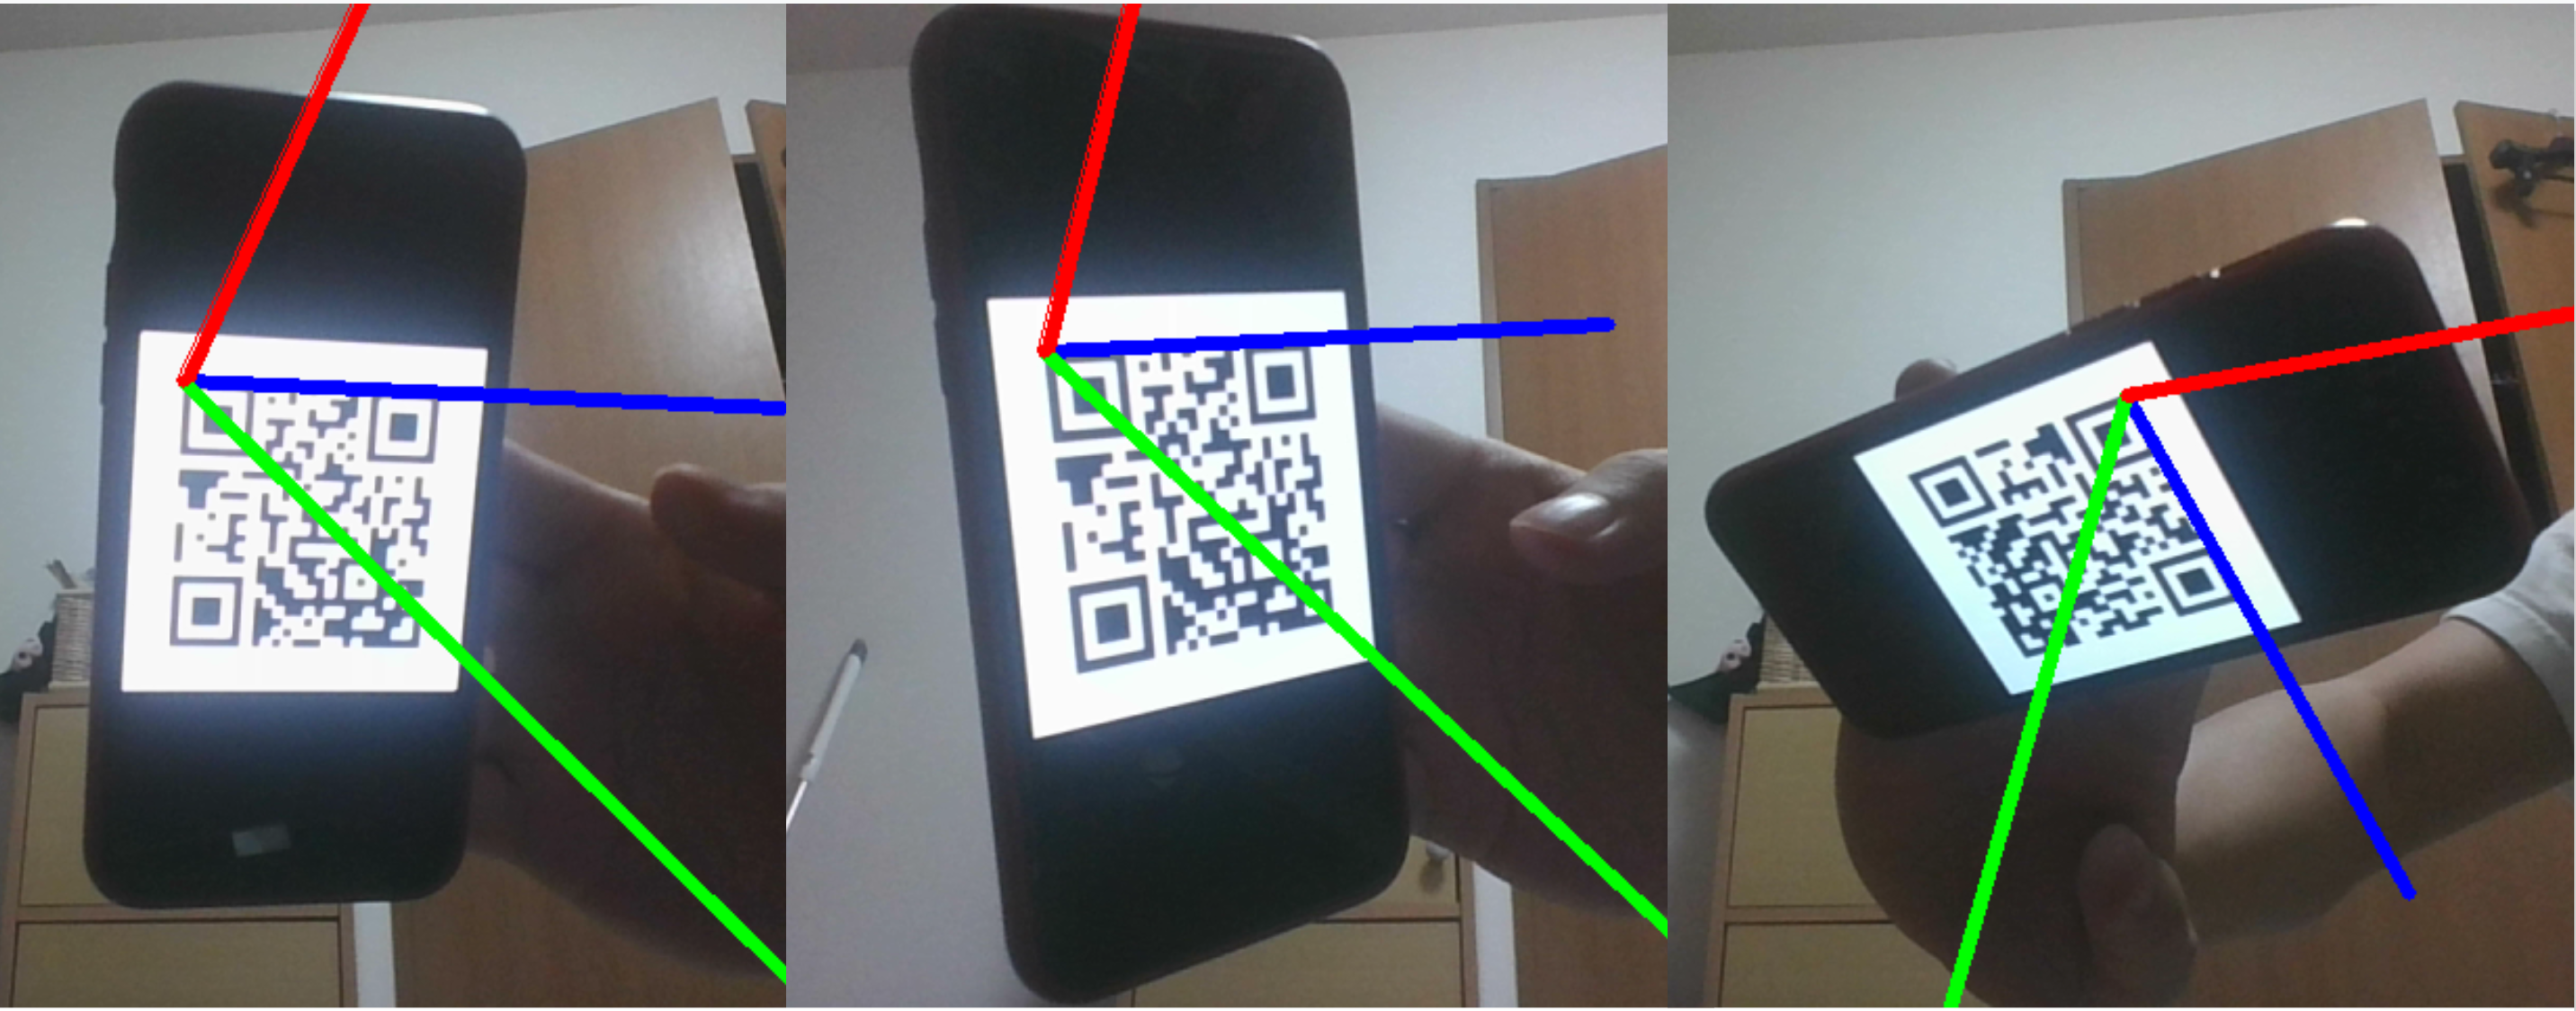
\includegraphics[clip,width=15.0cm]{img/pnp_qr.png}
    \caption{QRコードの姿勢推定}
    \label{fig:pnp_qr_img}
  \end{center}
\end{figure}
